\section{Testing the Terrain Hypothesis}
\label{sec:terrain}

Larger reconstruction error need not imply a larger correctable fraction. We
compare both against actual-orography roughness and retain the original
proxy-elevation comparison as a sensitivity check.

\subsubsection{Actual orography and roughness.}
ERA5 surface geopotential and land--sea mask are extracted from ARCO-ERA5 at
2018-01-01 00 UTC, with coordinates checked against the original $97\times241$
grid. Elevation is geopotential divided by $9.80665\,\mathrm{m\,s^{-2}}$; land
is $\mathrm{lsm}>0.5$. Roughness is population elevation standard deviation in a
$5\times5$ land-only neighbourhood with at least 13 valid neighbours. Ocean and
out-of-domain cells are excluded without padding. Excluding 102 land cells leaves
15{,}343 cells overall and 7{,}573 west of $100^\circ$W.

Ten terrain-only quantile bins per region fix identical cells before and after
correction. Per-channel normalised squared error is pooled over bin cells and
all 1{,}460 test frames, square-rooted, then averaged over the 19 direct channels.
The frozen checkpoint and 2014--2016 normalisation are unchanged.

\begin{figure}[t]
\centering
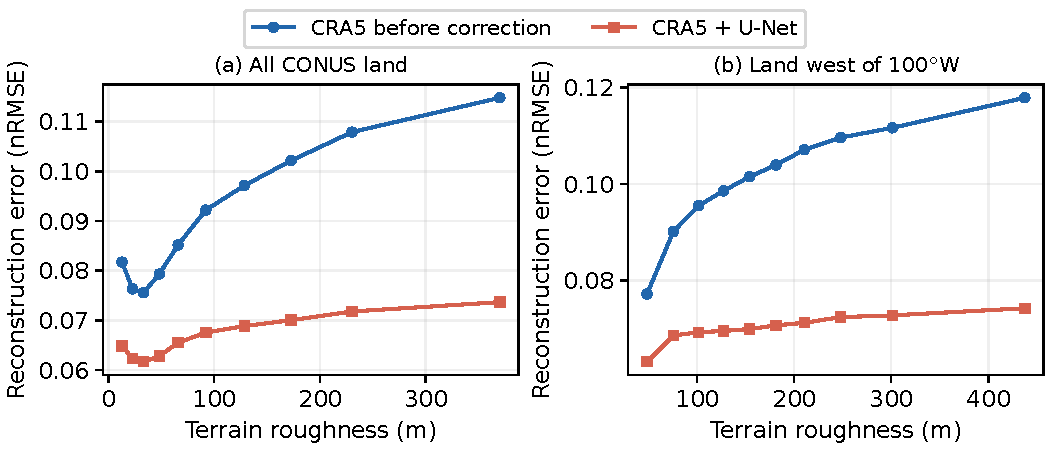
\includegraphics[width=\textwidth]{figs/terrain_roughness_main_curve}
\caption{2018 frozen U-Net errors: 19 direct channels, 2014--2016 normalisation.
Roughness is $5\times5$ land-only elevation SD with at least 13 valid neighbours.
Points are ten region-specific quantile bins at mean roughness; lines connect
measurements. Both curves use identical cells/timestamps within each panel.
Western land controls east--west composition; association does not imply causality.}
\label{fig:roughness}
\end{figure}

Figure~\ref{fig:roughness} shows larger baseline errors on rougher ground,
except for a non-monotone low-roughness segment on all land. Between endpoint
all-land deciles, baseline nRMSE rises from 0.08170 to 0.11482 and corrected
nRMSE from 0.06479 to 0.07364; $G$ rises from 20.7\% to 35.9\%. On western
land, baseline nRMSE rises from 0.07724 to 0.11783. Corrected error rises from
0.06323 to 0.07430; $G$ increases from 18.1\% to 36.9\%. Correction narrows but
does not remove the error gradient. All-land near-surface gain rises from 26.1\%
to 43.6\%; upper-air gains remain 3.1--3.7\% across deciles.

\subsubsection{Elevation controls.}
Roughness/elevation Spearman correlation is 0.694 overall and 0.265 on western
land. Western comparisons within fixed elevation bands (0--200, 200--600,
600--1200, 1200--2000, and above 2000\,m) retain the broad association in several
bands. For example, $G$ rises from 14.3\% to 36.8\% across endpoint deciles
at 600--1200\,m. The pattern is not uniform: 0--200\,m gains fluctuate around
30--35\%, with only 29--31 cells per bin. These are descriptive controls, not
independent spatial replications.

\subsubsection{Original proxy-elevation sensitivity.}
Table~\ref{tab:twoheights} retains the original comparison at fixed western
proxy-land positions.

\begin{table}[!htb]
\centering
\caption{Original elevation control, western proxy-land, 2018: identical ground
grid columns for near13/upper6, excluding \texttt{tcwv}. Gains are
$1-\sqrt{\langle a^2\rangle/\langle b^2\rangle}$, where $a,b$ are per-cell
normalised RMSE after/before correction; averaging pools channels and cells.
This differs from $G,\bar G$; ratios use unrounded gains.}
\label{tab:twoheights}
\begin{tabular}{lrrrr}
\toprule
Elevation band & Cells & Near & Upper & Ratio \\
\midrule
0--200\,m & 415 & 39.9\% & 5.0\% & 7.9$\times$ \\
200--600\,m & 850 & 39.2\% & 5.2\% & 7.6$\times$ \\
600--1200\,m & 2{,}311 & 33.5\% & 4.7\% & 7.1$\times$ \\
1200--2000\,m & 3{,}113 & 40.1\% & 4.7\% & 8.6$\times$ \\
above 2000\,m & 984 & \textbf{41.9\%} & \textbf{4.3\%} & \textbf{9.7$\times$} \\
\bottomrule
\end{tabular}
\end{table}

The pressure-derived standard-atmosphere elevation and 1.0\,K diurnal
2\,m-temperature land threshold differ from the actual static fields above.
The baseline surface-pressure high/low-elevation error ratio is $3.23\times$
over CONUS, $2.28\times$ on proxy-land, and $1.14\times$ on western proxy-land;
MPCA+PCA e995 gives 2.09, 1.70, and 0.95. This negative result is retained:
mean elevation differs from roughness, and the original gradient is strongly
confounded by land/sea and longitude.

Above 2000\,m, eight low-level channels may include below-ground ERA5
extrapolation, potentially easing prediction. Proxy-sea gains also differ,
23.9\% versus 5.5\%: ground location alone does not explain the split.
